% Session 4 - Money-laundering patterns in a transaction graph.
% Build:  pdflatex Fig-AMLPatterns.tex
%         pdf2svg Fig-AMLPatterns.pdf Fig-AMLPatterns.svg
\documentclass[tikz,border=10pt]{standalone}
\usepackage{tikz}
\usepackage{amsmath,amssymb}
\usepackage[T1]{fontenc}
\usepackage{lmodern}
\usepackage{microtype}
\usetikzlibrary{positioning,arrows.meta,shapes.geometric,calc,backgrounds,fit,shadows.blur}

% --- Palette: same family as the S2 canonical figure ---
\definecolor{legitBorder}{HTML}{1E40AF}    \definecolor{legitFill}{HTML}{DBEAFE}
\definecolor{fraudBorder}{HTML}{B31B1B}    \definecolor{fraudFill}{HTML}{FEE2E2}
\definecolor{muleBorder}{HTML}{B45309}     \definecolor{muleFill}{HTML}{FEF3C7}
\definecolor{srcBorder}{HTML}{5B21B6}      \definecolor{srcFill}{HTML}{EDE9FE}

\definecolor{ink}{HTML}{1F2937}
\definecolor{rule}{HTML}{4B5563}
\definecolor{paper}{HTML}{FFFFFF}

\begin{document}
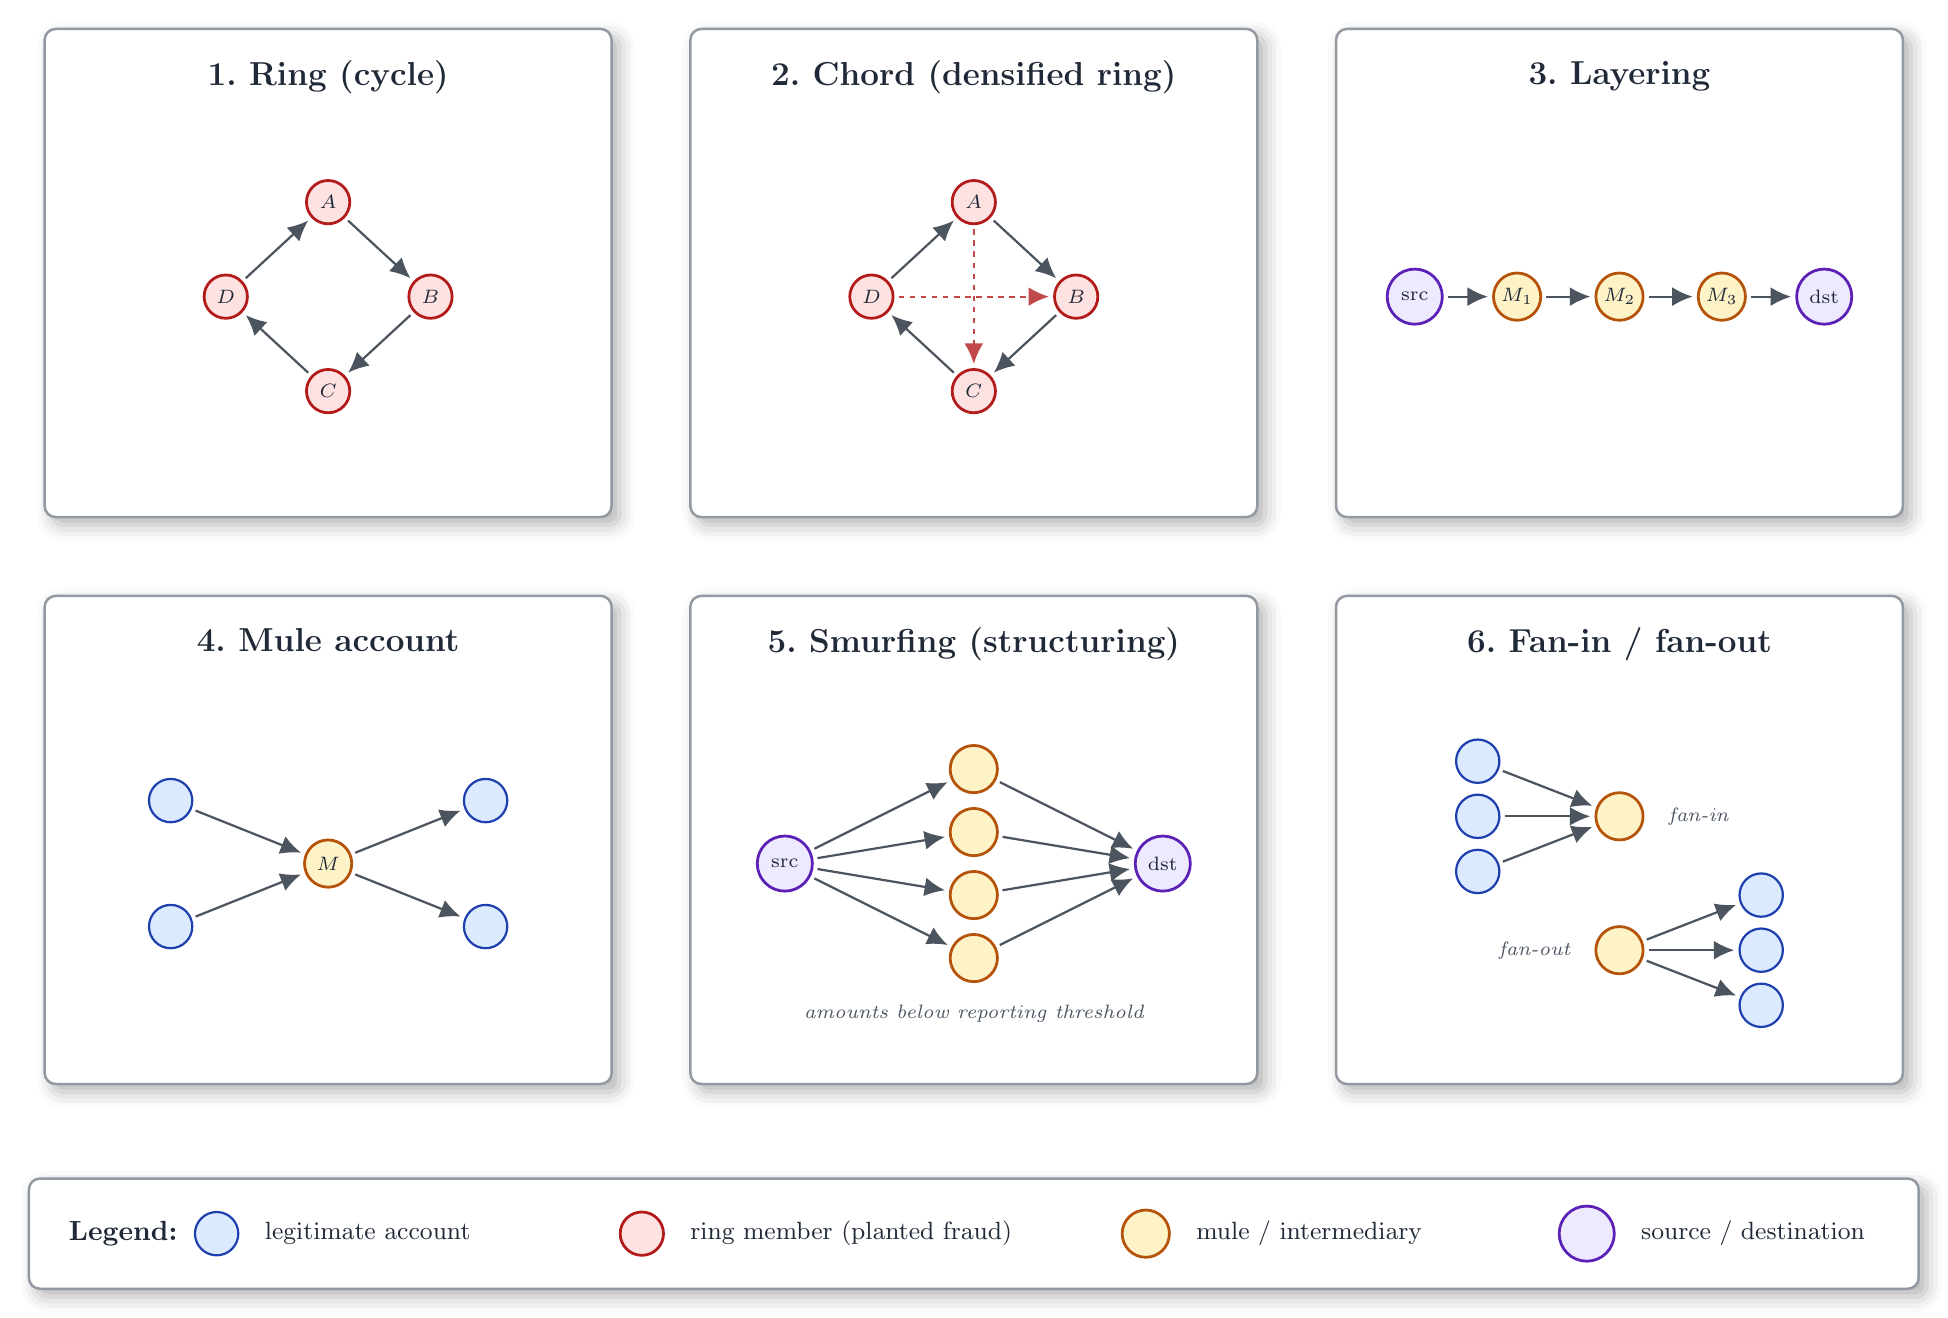
\begin{tikzpicture}[
    >={Latex[length=2.6mm,width=2.4mm]},
    every node/.style={font=\footnotesize, text=ink},
    panel/.style={
        rectangle, rounded corners=4pt, line width=0.9pt,
        draw=rule!60, fill=paper,
        minimum width=72mm, minimum height=62mm,
        blur shadow={shadow xshift=1.0mm, shadow yshift=-1.0mm,
                     shadow opacity=30, shadow blur radius=2mm},
    },
    paneltitle/.style={font=\large\bfseries\scshape, text=ink, anchor=north},
    legit/.style={circle, draw=legitBorder, fill=legitFill, line width=0.8pt,
                  minimum size=5.5mm, inner sep=0pt, font=\scriptsize},
    fraud/.style={circle, draw=fraudBorder, fill=fraudFill, line width=1pt,
                  minimum size=5.5mm, inner sep=0pt, font=\scriptsize},
    mule/.style={circle, draw=muleBorder, fill=muleFill, line width=1pt,
                 minimum size=6mm, inner sep=0pt, font=\scriptsize},
    src/.style={circle, draw=srcBorder, fill=srcFill, line width=1pt,
                minimum size=7mm, inner sep=0pt, font=\scriptsize},
    edge/.style={->, line width=0.8pt, draw=ink!80, shorten >=1.5pt, shorten <=1.5pt},
    chord/.style={->, line width=0.8pt, draw=fraudBorder!80,
                  dash pattern=on 2pt off 2pt, shorten >=1.5pt, shorten <=1.5pt},
]

\def\dx{82mm}
\def\dy{72mm}

% =========== Panel 1: Ring ===========
\node[panel] (P1) at (0,0) {};
\node[paneltitle] at ([yshift=-3mm]P1.north) {1.\ Ring (cycle)};
\begin{scope}[shift={(0,-3mm)}]
    \node[fraud] (r1) at ( 0mm, 12mm) {$A$};
    \node[fraud] (r2) at (13mm,  0mm) {$B$};
    \node[fraud] (r3) at ( 0mm,-12mm) {$C$};
    \node[fraud] (r4) at (-13mm, 0mm) {$D$};
    \draw[edge] (r1) -- (r2);
    \draw[edge] (r2) -- (r3);
    \draw[edge] (r3) -- (r4);
    \draw[edge] (r4) -- (r1);
\end{scope}

% =========== Panel 2: Chord ===========
\node[panel] (P2) at (\dx,0) {};
\node[paneltitle] at ([yshift=-3mm]P2.north) {2.\ Chord (densified ring)};
\begin{scope}[shift={(\dx,-3mm)}]
    \node[fraud] (s1) at ( 0mm, 12mm) {$A$};
    \node[fraud] (s2) at (13mm,  0mm) {$B$};
    \node[fraud] (s3) at ( 0mm,-12mm) {$C$};
    \node[fraud] (s4) at (-13mm, 0mm) {$D$};
    \draw[edge] (s1) -- (s2);
    \draw[edge] (s2) -- (s3);
    \draw[edge] (s3) -- (s4);
    \draw[edge] (s4) -- (s1);
    \draw[chord] (s1) -- (s3);
    \draw[chord] (s4) -- (s2);
\end{scope}

% =========== Panel 3: Layering ===========
\node[panel] (P3) at (2*\dx,0) {};
\node[paneltitle] at ([yshift=-3mm]P3.north) {3.\ Layering};
\begin{scope}[shift={(2*\dx - 26mm,-3mm)}]
    \node[src]   (l0) at ( 0mm, 0) {src};
    \node[mule]  (l1) at (13mm, 0) {$M_1$};
    \node[mule]  (l2) at (26mm, 0) {$M_2$};
    \node[mule]  (l3) at (39mm, 0) {$M_3$};
    \node[src]   (l4) at (52mm, 0) {dst};
    \draw[edge] (l0) -- (l1);
    \draw[edge] (l1) -- (l2);
    \draw[edge] (l2) -- (l3);
    \draw[edge] (l3) -- (l4);
\end{scope}

% =========== Panel 4: Mule accounts ===========
\node[panel] (P4) at (0,-\dy) {};
\node[paneltitle] at ([yshift=-3mm]P4.north) {4.\ Mule account};
\begin{scope}[shift={(0,-\dy - 3mm)}]
    \node[legit] (a1) at (-20mm,  8mm) {};
    \node[legit] (a2) at (-20mm, -8mm) {};
    \node[mule]  (mm) at (  0mm,  0mm) {$M$};
    \node[legit] (b1) at ( 20mm,  8mm) {};
    \node[legit] (b2) at ( 20mm, -8mm) {};
    \draw[edge] (a1) -- (mm);
    \draw[edge] (a2) -- (mm);
    \draw[edge] (mm) -- (b1);
    \draw[edge] (mm) -- (b2);
\end{scope}

% =========== Panel 5: Smurfing ===========
\node[panel] (P5) at (\dx,-\dy) {};
\node[paneltitle] at ([yshift=-3mm]P5.north) {5.\ Smurfing (structuring)};
\begin{scope}[shift={(\dx,-\dy - 3mm)}]
    \node[src]   (sm0) at (-24mm,  0mm) {src};
    \node[mule]  (sm1) at (  0mm, 12mm) {};
    \node[mule]  (sm2) at (  0mm,  4mm) {};
    \node[mule]  (sm3) at (  0mm, -4mm) {};
    \node[mule]  (sm4) at (  0mm,-12mm) {};
    \node[src]   (sm5) at ( 24mm,  0mm) {dst};
    \draw[edge] (sm0) -- (sm1);
    \draw[edge] (sm0) -- (sm2);
    \draw[edge] (sm0) -- (sm3);
    \draw[edge] (sm0) -- (sm4);
    \draw[edge] (sm1) -- (sm5);
    \draw[edge] (sm2) -- (sm5);
    \draw[edge] (sm3) -- (sm5);
    \draw[edge] (sm4) -- (sm5);
    \node[font=\scriptsize\itshape, text=rule] at (0,-19mm)
         {amounts below reporting threshold};
\end{scope}

% =========== Panel 6: Fan-in / Fan-out ===========
\node[panel] (P6) at (2*\dx,-\dy) {};
\node[paneltitle] at ([yshift=-3mm]P6.north) {6.\ Fan-in / fan-out};
\begin{scope}[shift={(2*\dx,-\dy)}]
    % Fan-in (top half)
    \node[legit] (fi1) at (-18mm,  10mm) {};
    \node[legit] (fi2) at (-18mm,   3mm) {};
    \node[legit] (fi3) at (-18mm,  -4mm) {};
    \node[mule]  (fih) at (  0mm,   3mm) {};
    \draw[edge] (fi1) -- (fih);
    \draw[edge] (fi2) -- (fih);
    \draw[edge] (fi3) -- (fih);
    \node[font=\scriptsize\itshape, text=rule, anchor=west] at (5mm,3mm) {fan-in};
    % Fan-out (bottom half)
    \node[mule]  (foh) at (  0mm, -14mm) {};
    \node[legit] (fo1) at ( 18mm, -7mm) {};
    \node[legit] (fo2) at ( 18mm,-14mm) {};
    \node[legit] (fo3) at ( 18mm,-21mm) {};
    \draw[edge] (foh) -- (fo1);
    \draw[edge] (foh) -- (fo2);
    \draw[edge] (foh) -- (fo3);
    \node[font=\scriptsize\itshape, text=rule, anchor=east] at (-5mm,-14mm) {fan-out};
\end{scope}

% =========== Legend ===========
\node[panel, minimum width=240mm, minimum height=14mm] (LEG)
    at (\dx, -\dy - 50mm) {};
\node[font=\bfseries\scshape, text=ink, anchor=west]
    at ([xshift=4mm,yshift=0mm]LEG.west) {Legend:};
\node[legit] (lg1) at ($(LEG.west) + (24mm,0)$) {};
\node[anchor=west, font=\small] at ($(lg1.east)+(2mm,0)$) {legitimate account};
\node[fraud] (lg2) at ($(LEG.west) + (78mm,0)$) {};
\node[anchor=west, font=\small] at ($(lg2.east)+(2mm,0)$) {ring member (planted fraud)};
\node[mule]  (lg3) at ($(LEG.west) + (142mm,0)$) {};
\node[anchor=west, font=\small] at ($(lg3.east)+(2mm,0)$) {mule / intermediary};
\node[src]   (lg4) at ($(LEG.west) + (198mm,0)$) {};
\node[anchor=west, font=\small] at ($(lg4.east)+(2mm,0)$) {source / destination};

\end{tikzpicture}
\end{document}
